\subsection{Twitter Analysis}

When, the classifier engine was created, we also managed to have enough tweets to perform analysis on our corpus.  

\vbox to 0.2cm{}
{\bf Challenge 2: Size of Data}

One of the biggest challenges was the size of the data. First, we tried working directly with the database,
creating a new view in CouchDB for every experiment. These views used MapReduce algorithm. This turned out to be too slow to be usable, because every
time a view is created or updated, it needs to be reindexed. So even just a forgotten letter
in a hashtag or parenthesis in the code, lead to a couple of minutes of waiting.


Subsequently, we tried to filter tweets locally for the purpose of analysis. At this stage,
jupyter notebook turned out to be very useful, because it allows rerun only parts of the code without
the need to wait for other parts of the code. So we created a loop
in Python to fetch them tweet by tweet and then throw away those we did not need. Unfortunately, this was even slower.

Finally, we decided to download all data locally and use utilities like grep, to observe the data and find a story. The resulting file was about 200 MB big and as such it was fairly fast and easy to work with it locally. We are aware of the fact that it is not a scallable solution to
download all data, but the idea is to download only representative sample to find a story in it and 
once the story is agreed upon, we can deploy MapReduce view and other logic directly on our servers.

\vbox to 0.2cm{}
{\bf Challenge 3: Lack of Tweets Being Classified}

When passing the engine to filter tweets that weren’t based on wrath, we were able to get a very small set of tweets that had the wrath sentiment. We realized soon enough that these tweets won’t be enough to validate our story using AURIN. We even tried populating our list on synonyms with slang words expressed in tweets but we were still not able to extract enough tweets.One of the ways to overcome the wrath scenario was to consider multiple sentiments in a text rather than just trying to classify a text whether it denoted wrath (anger) or not. Through our research, we came across a familiar approach in \footnote{\url{http://nil.fdi.ucm.es/sites/default/files/FranciscoEtAlNovaSW.pdf}}. The approach relied upon creating ontology. The ontology consisted of some basic emotional categories such as Anger, Fear, Happy, Sad and Surprise. Then, emotional dimensions were used to quantify emotions into numeric value. The way the emotional dimensions work is by using three functions that allows us to calculate an evaluation score, activation score and a power score. Evaluation represents how positive or negative an emotion is. At one extreme we have emotions such as happiness, satisfaction and hope while at the other we find emotions such as unhappiness, un-satisfaction and desperation. Activation represents an activity versus passivity scale of emotions, with emotions such as excitation at one extreme, and arousal and at the other emotions such as calm and relaxation. Power represents the sense of control which the emotion exerts on the subject. At one end of the scale we have emotions characterized as completely controlled, such as fear and submission and at the other end we find emotions such as dominance and contempt. And by having ranges for our root emotional categories, the approach ended up assigning all other words to one of these emotions to create an ontology. An illustration of ontology is shown in figure 18. 

Our assumption was that if we were able to give scores for each emotion in a subjective text and then only take tweets that had the highest value of anger emotion, we may get more tweets that may show anger/wrath. We even sent a request to the Universidad Complutense de Madrid to give us access to their ontology.



\begin{figure}[H]
    \centering
    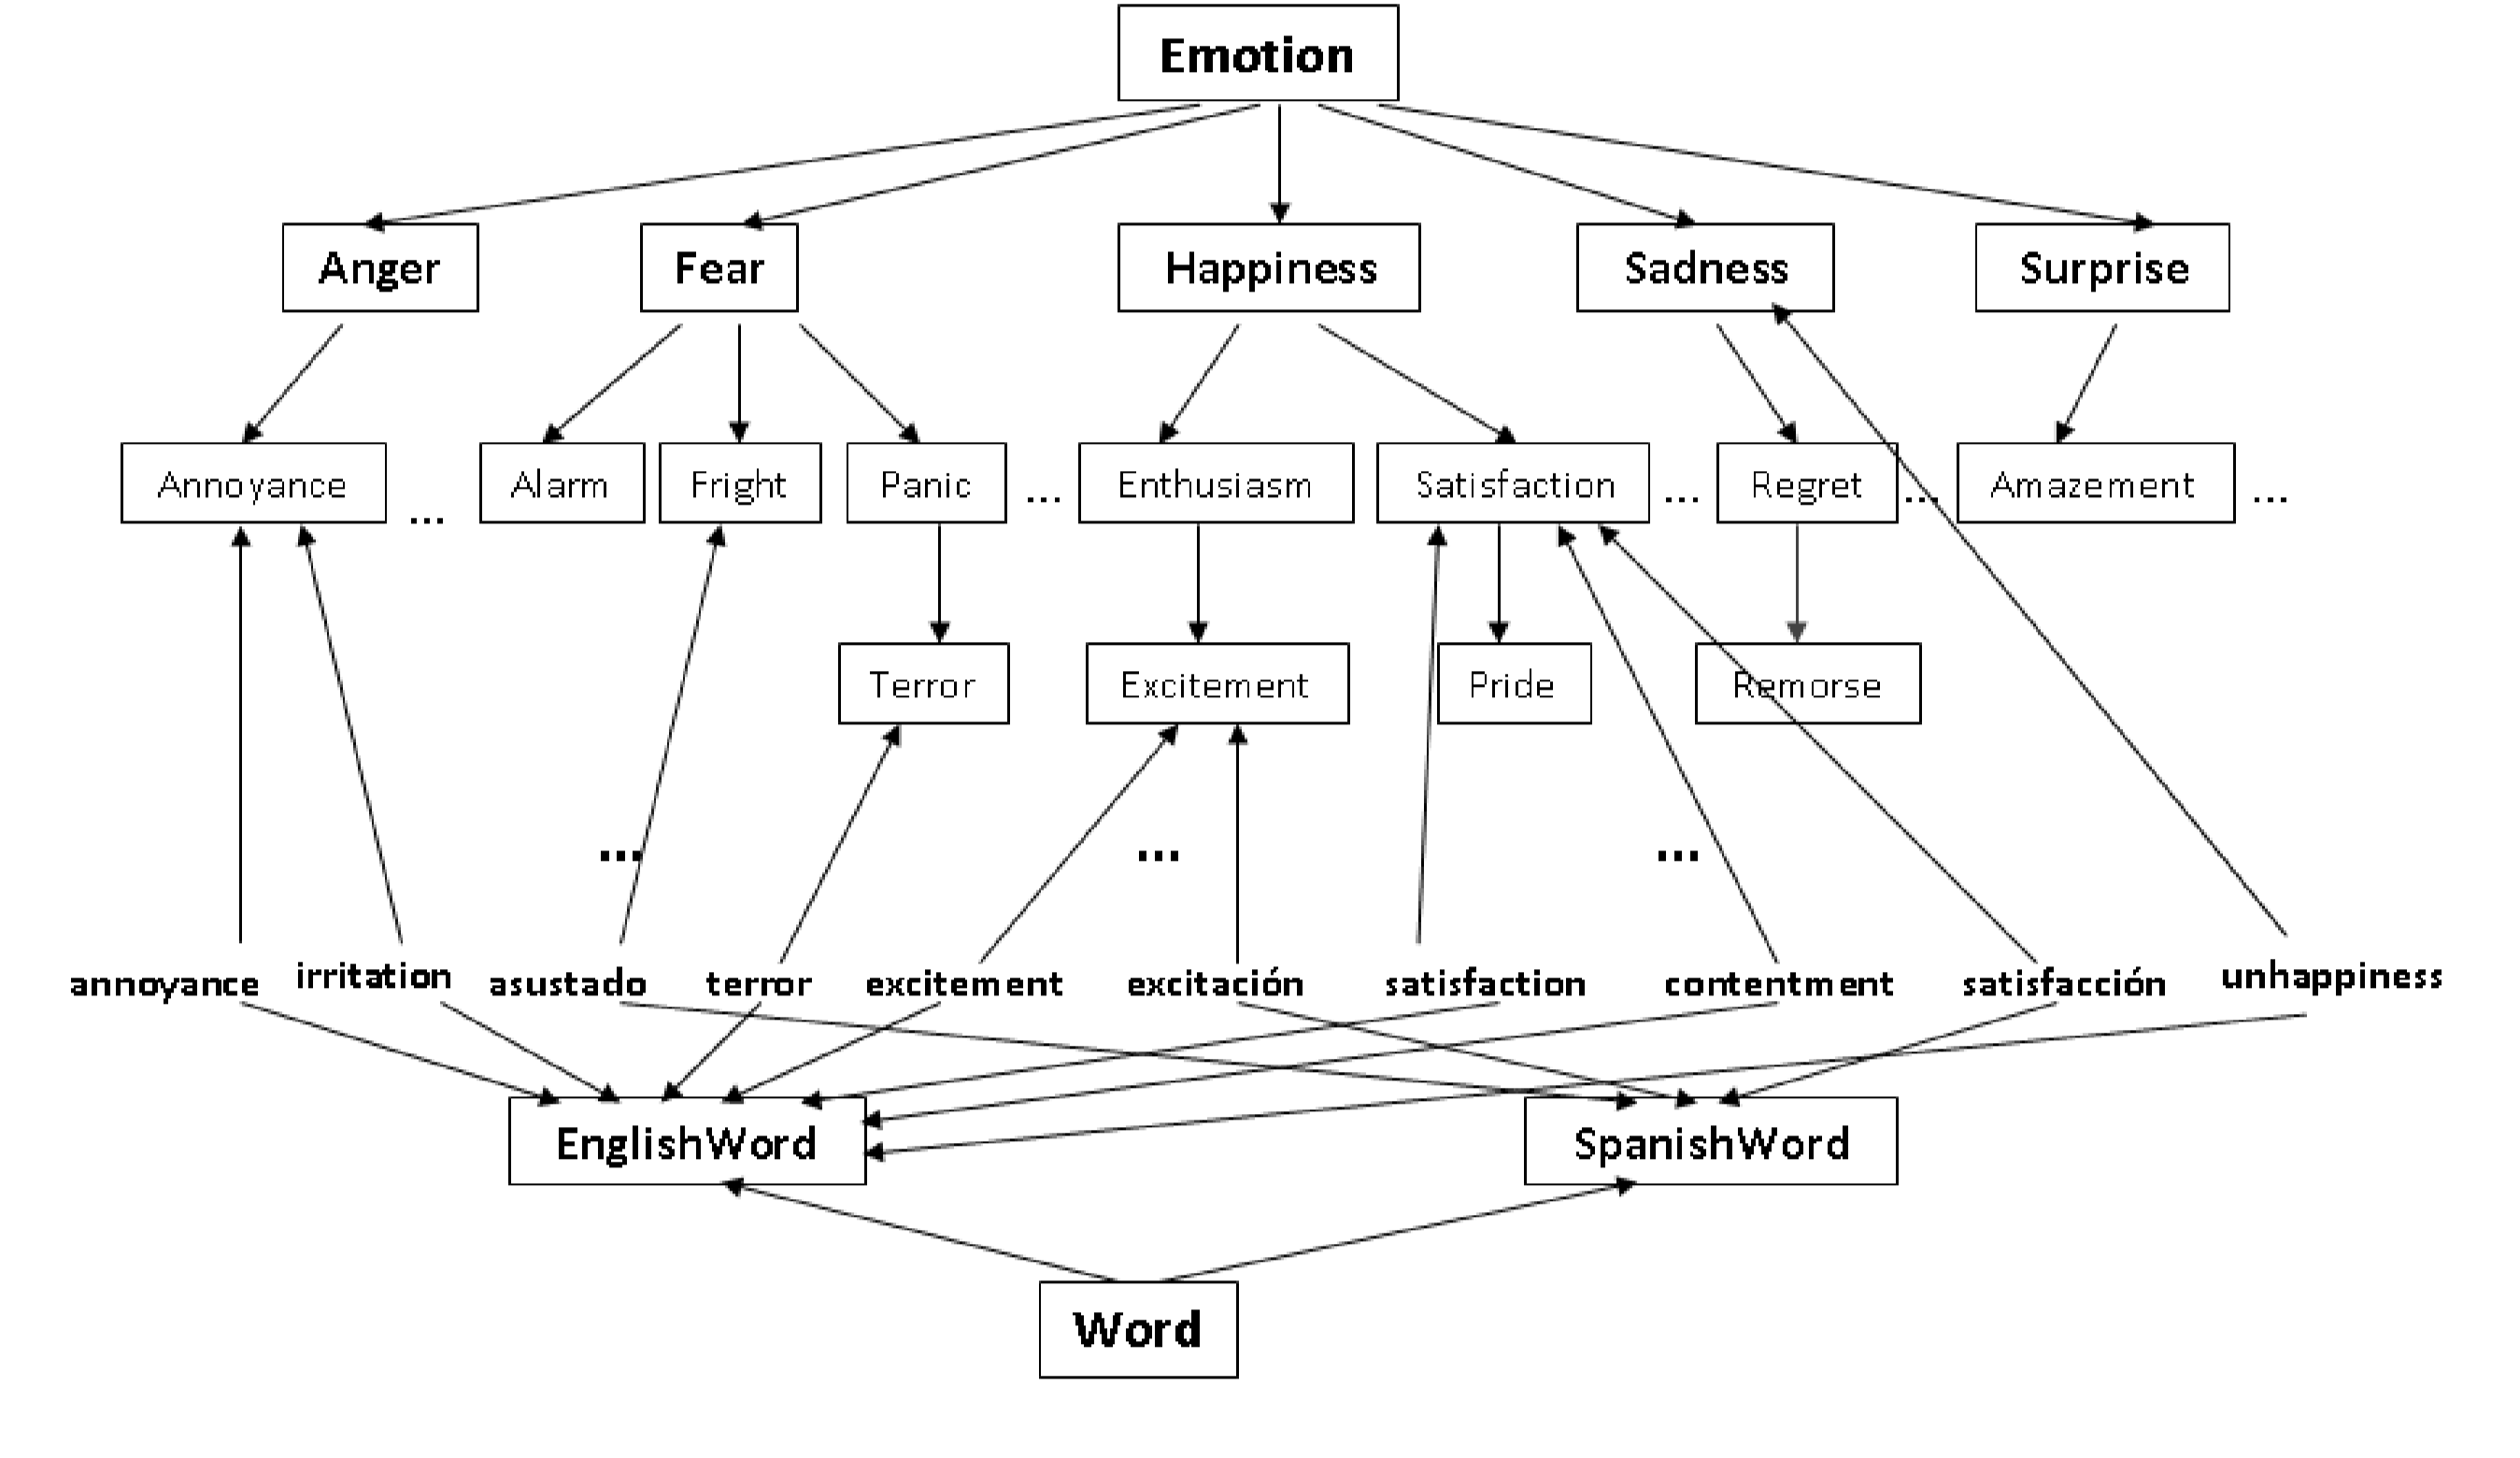
\includegraphics[width=12cm,keepaspectratio=true]{images/deployment/Tree_OntoEmotion.png}
    \caption{Ontology Architecture}
    \label{fig:ontology architecture}
\end{figure}
 
\subsubsection{Changing The Story Line}

While waiting for the ontology, we also tried different approaches.
There were many ideas around crime or alcohol consumption, but it was hard to find a correlation with real data. There are many reasons for that. Some areas are more densely populated, some have more bars and many analysis just ended up having most tweets around CBD and the farther we went, the fewer tweets appeared.

\vbox to 0.2cm{}
{\bf Supervised Learner}

The first idea was to get some data to train a supervised learner. FastText\footnote{\url{https://fasttext.cc/}} would be especially handy for this. The problem was that we had to build a corpus. We tried to get some tweets expressing clearly wrath and manually label these as positive samples. Then we were hoping to correlate them with the data from AURIN regarding the perception of safety in the streets in different areas of Melbourne.

We tried to automatically tweets containing particular phrases or hashtags, because it is unfeasible to go through about 300.000 tweets we had at the time manually. Getting tweets containing phrases like ``fear'' did not help at all, because we got tweets not connected to wrath at all (An example is ``Fear is Good.``).

Because we could not build a sufficient corpus for training a learner, we decided to go a simpler way.

\vbox to 0.2cm{}
{\bf The Final Story}


This time we actually tried to analyze the corpus we had to understand the content. To do this we went through about 10 thousand tweets to understand the most frequent words in the corpus. Interestingly, we saw that there were a large number of tweets that revolved around keywords: ‘food’, ‘drink’, ‘cafe’, ‘restaurant’, etc. These tweets predominantly revolved around gluttony. We also came across a dataset in Local Government Area (LGA) profiles data for VIC. This dataset contained the percentage of people having diabetes, high blood pressure, obesity and heart diseases in certain parts of victoria. Since, most of the tweets were being harvested from Melbourne, we targeted only Melbourne. While extracting tweets on gluttony based on the above keywords, we were able to get decent correlation between the ratio of tweets and the people having such diseases. 

After completing our correlation, we were also presented with the ontology from Universidad Complutense de Madrid. However, due to limitation in time for submission, we haven’t been able to explore our previous story line using the ontology. We plan to use the ontology to complete our analysis in due time.

As we had many tries and a lot of code, we decided to merge only the used code. Not used parts can be found in branches {\it knezi-analyse} and {\it kabir-branch}.